% Drawing 142/06-15 -- folder 142, batch 06, archive page 113 (PDF page 114).
% Transcription: À gauche, un morceau de carte et sa subdivision barycentrique : sommets marqués $0$, $1$, $\infty$, le triangle central $r$ (entouré) avec ses sommets $R^0_r$, $R^1_r$, $R^\infty_r$ et ses côtés $a^0_r$, $a^1_r$, $a^\infty_r$, $\lambda^0_r$, $\lambda^1_r$, $\lambda^\infty_r$ ; les triangles voisins sont étiquetés $\tau_0(r)$, $\tau_1(r)$, $\tau_\infty(r)$ (signe $-$), $\rho_\infty(r) = \tau_1\tau_0(r)$, $\rho_\infty^{-1}(r) = \tau_0(\tau_1(r))$, $\tau_\infty\tau_1(r) = \rho_0(r)$, $\tau_1\tau_\infty(r) = \rho_0^{-1}(r)$, $\rho_1(r) = \tau_0\tau_\infty(r) = \tau_\infty\tau_0(r)$ (signe $+$) ; les points $R_f$ ($\infty$), $R_s$ ($0$), $R_a$ ($1$), $R^{0,1}_r$, $R^{1,\infty}_r$, $R^{0,\infty}_r$ ; flèches courbes de rotation autour des sommets.
% Kind: piece of a map with its barycentric subdivision and labelled triangles. Method 2 (schematic redraw from the facsimile). Status: partial.
% Notes: A piece of a map (vertices 0, 1, infinity) with its barycentric subdivision: the central triangle r (ringed) with R^0_r, R^1_r, R^infty_r, the sides a^i_r and lambda^i_r; the neighbouring triangles labelled tau_0(r), tau_1(r), tau_infty(r) (sign -) and rho_infty(r) = tau_1 tau_0(r), rho_infty^{-1}(r) = tau_0(tau_1(r)), tau_infty tau_1(r) = rho_0(r), rho_1(r) = tau_0 tau_infty(r) = tau_infty tau_0(r) (sign +); the points R_f (infinity), R_s (0), R_a (1), R^{0,1}_r, R^{1,infty}_r, R^{0,infty}_r. The inked strokes and arrows are drawn schematically (their exact course and every arrowhead are not reproduced); pencil strokes of the subdivision partly omitted. The label tau_1 tau_infty(r) = rho_0^{-1}(r) is not found on the crop.
% Coordinates: 1 unit = 1 mm = 1/100 of the crop width (bbox in page fractions: [0.22, 0.36, 0.62, 0.645]).
% Redrawn by Claude (claude-opus-5-5), issue #73, 2026-11-07; not checked by a human; not compiled (no TeX in the session).
% Rights: reproduces part of the work -- behind RENDER_TRANSCRIPTS, never published by itself.
\documentclass[tikz,border=3pt]{standalone}
\usepackage{amsmath,amssymb}
\usetikzlibrary{patterns,arrows.meta}
\tikzset{pencil/.style={black!45}, struck/.style={black!35}, mark/.style={circle,draw,inner sep=1.3pt}, pt/.style={circle,fill,inner sep=0.9pt}, opt/.style={circle,draw,fill=white,inner sep=1.1pt}}
\begin{document}
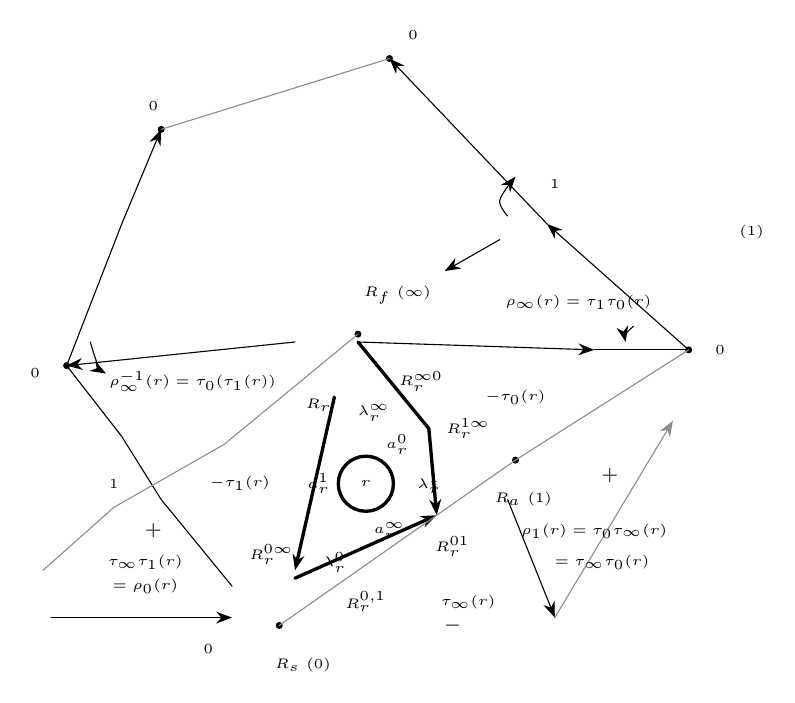
\begin{tikzpicture}[x=1mm,y=1mm,line cap=round,line join=round,font=\scriptsize]
\node[pt] at (20,-23) {};
\node[pt] at (49,-14) {};
\node[pt] at (8,-53) {};
\node[pt] at (87,-51) {};
\node[pt] at (45,-49) {};
\node[pt] at (65,-65) {};
\node[pt] at (35,-86) {};
\draw[-{Stealth[length=2mm]}] (8,-53) -- (15,-35) -- (20,-23);
\draw[pencil] (20,-23) -- (49,-14);
\draw[{Stealth[length=2mm]}-] (49,-14) -- (69,-35);
\draw[{Stealth[length=2mm]}-] (69,-35) -- (87,-51);
\draw[{Stealth[length=2mm]}-] (8,-53) -- (37,-50);
\draw[-{Stealth[length=2mm]}] (45,-50) -- (75,-51);
\draw (75,-51) -- (87,-51);
\draw (8,-53) -- (15,-62) -- (20,-70) -- (29,-81);
\draw[pencil] (45,-49) -- (28,-63) -- (14,-71);
\draw[pencil] (14,-71) -- (5,-79);
\draw[very thick] (45,-50) -- (54,-61);
\draw[very thick,-{Stealth[length=2mm]}] (54,-61) -- (55,-72);
\draw[very thick,-{Stealth[length=2mm]}] (42,-57) -- (37,-79);
\draw[very thick,-{Stealth[length=2mm]}] (37,-80) -- (55,-72);
\draw[pencil] (35,-86) -- (65,-65);
\draw[pencil] (65,-65) -- (87,-51);
\draw[-{Stealth[length=2mm]}] (64,-70) -- (70,-85);
\draw[pencil,-{Stealth[length=2mm]}] (70,-85) -- (85,-60);
\draw[-{Stealth[length=2mm]}] (6,-85) -- (29,-85);
\draw[-{Stealth[length=2mm]}] (63,-37) -- (56,-41);
\draw[very thick] (46,-68) circle[radius=3.5];
\draw[-{Stealth[length=2mm]}] plot[smooth, tension=0.55] coordinates {(11,-50) (12,-53) (13,-54)};
\draw[-{Stealth[length=2mm]}] plot[smooth, tension=0.55] coordinates {(64,-34) (63,-32) (65,-29)};
\draw[-{Stealth[length=2mm]}] plot[smooth, tension=0.55] coordinates {(80,-48) (79,-49) (79,-50)};
\node[inner sep=1pt] at (19,-20) {\tiny $0$};
\node[inner sep=1pt] at (52,-11) {\tiny $0$};
\node[inner sep=1pt] at (4,-54) {\tiny $0$};
\node[inner sep=1pt] at (91,-51) {\tiny $0$};
\node[inner sep=1pt] at (70,-30) {\tiny $1$};
\node[inner sep=1pt] at (14,-68) {\tiny $1$};
\node[inner sep=1pt] at (26,-89) {\tiny $0$};
\node[inner sep=1pt] at (95,-36) {\tiny (1)};
\node[inner sep=1pt] at (50,-44) {\tiny $R_f\ (\infty)$};
\node[inner sep=1pt] at (73,-45) {\tiny $\rho_\infty(r)=\tau_1\tau_0(r)$};
\node[inner sep=1pt] at (24,-55) {\tiny $\rho_\infty^{-1}(r)=\tau_0(\tau_1(r))$};
\node[inner sep=1pt] at (40,-58) {\tiny $R_r$};
\node[inner sep=1pt] at (53,-55) {\tiny $R^{\infty0}_r$};
\node[inner sep=1pt] at (47,-59) {\tiny $\lambda^\infty_r$};
\node[inner sep=1pt] at (65,-57) {\tiny $-\tau_0(r)$};
\node[inner sep=1pt] at (50,-63) {\tiny $a^0_r$};
\node[inner sep=1pt] at (59,-61) {\tiny $R^{1\infty}_r$};
\node[inner sep=1pt] at (30,-68) {\tiny $-\tau_1(r)$};
\node[inner sep=1pt] at (40,-68) {\tiny $a^1_r$};
\node[inner sep=1pt] at (46,-68) {\tiny $r$};
\node[inner sep=1pt] at (54,-68) {\tiny $\lambda^1_r$};
\node[inner sep=1pt] at (66,-70) {\tiny $R_a\ (1)$};
\node[inner sep=1pt] at (77,-67) {\scriptsize $+$};
\node[inner sep=1pt] at (75,-74) {\tiny $\rho_1(r)=\tau_0\tau_\infty(r)$};
\node[inner sep=1pt] at (76,-78) {\tiny $=\tau_\infty\tau_0(r)$};
\node[inner sep=1pt] at (49,-74) {\tiny $a^\infty_r$};
\node[inner sep=1pt] at (57,-76) {\tiny $R^{01}_r$};
\node[inner sep=1pt] at (18,-78) {\tiny $\tau_\infty\tau_1(r)$};
\node[inner sep=1pt] at (18,-81) {\tiny $=\rho_0(r)$};
\node[inner sep=1pt] at (19,-74) {\scriptsize $+$};
\node[inner sep=1pt] at (34,-77) {\tiny $R^{0\infty}_r$};
\node[inner sep=1pt] at (42,-78) {\tiny $\lambda^0_r$};
\node[inner sep=1pt] at (46,-83) {\tiny $R^{0,1}_r$};
\node[inner sep=1pt] at (59,-83) {\tiny $\tau_\infty(r)$};
\node[inner sep=1pt] at (57,-86) {\scriptsize $-$};
\node[inner sep=1pt] at (38,-91) {\tiny $R_s\ (0)$};
\end{tikzpicture}
\end{document}
